\PassOptionsToPackage{dvipsnames}{xcolor}
\documentclass[
       embeddedlogo,
       english,
       lmodern,
       coorientadorbanca,
       noabntexcite
]{ufsc-thesis-rn46-2019}

\usepackage{thesis}
\usepackage{pdfpages}

%%%%%%%%%%%%%%%%%%%%%%%%%%%%%%%%%%%%%%%%%%%%%%%%%%%%%%%%%%%%%%%%%%%%
%%% Configurações da classe (dados do trabalho)                  %%%
%%%%%%%%%%%%%%%%%%%%%%%%%%%%%%%%%%%%%%%%%%%%%%%%%%%%%%%%%%%%%%%%%%%%

% Informações para capa e folha de rosto/certificacao

% Caso o título contenha alguma porção LaTeX ilegível, defina um título
% alternativo opcional com []'s para ser usado no campo Title do PDF
% IMPORTANTE: Os títulos deveriam ser iguais. Apenas use um título
% alternativo se o título não puder ser expresso com letras e números
\titulo[Implementing a programming language with a dependent type system]{Implementing a programming language with a dependent type system}

\autor{Eduardo Henke}
\data{\today}
\instituicao{Universidade Federal de Santa Catarina}
\centro{Centro Tecnológico}
\local{Florianópolis} % Apenas cidade! Sem estado
\programa{Programa de Pós-Graduação em Ciência da Computação}
% Os dois próximos itens são usados para gerar o \preambulo
% \tese % ou \dissertacao ou \tcc
% \titulode{graduação em Ciência da Computação}

%%% Atenção! No caso de TCC, além de usar \tcc, outros comandos devem ser fornecidos:
%%%
\tcc
\departamento{Departamento de Informática e Estatística}
\curso{Ciência da Computação}
\titulode{Bacharel em Ciência da Computação}

% Orientador, coorientador, membros da banca e coordenador
% As regras da BU agora exigem que Dr. apareça **depois** do nome
% Dica: para gerar Profᵃ. use Prof\textsuperscript{a}.
% Dica 2: para feminino use \orientadora e \coorientadora
\orientador{Prof. Alvaro Junio Pereira Franco, Dr.}
\coorientadorext{Li-Yao Xia, Dr.}{University of Edinburgh}
\membrabanca{Prof\textsuperscript{a}. Jerusa Marchi, Dr.}{Universidade Federal de Santa Catarina}
\membrobanca{Prof. Maicon Rafael Zatelli, Dr.}{Universidade Federal de Santa Catarina}
% Dica: se feminino, \coordenadora
\coordenador{Prof. Jean Everson Martina, Dr}

\begin{document}
%%%%%%%%%%%%%%%%%%%%%%%%%%%%%%%%%%%%%%%%%%%%%%%%%%%%%%%%%%%%%%%%%%%%
%%% Principais elementos pré-textuais                            %%%
%%%%%%%%%%%%%%%%%%%%%%%%%%%%%%%%%%%%%%%%%%%%%%%%%%%%%%%%%%%%%%%%%%%%

% Inicia parte pré-textual do documento capa, folha de rosto, folha de
% aprovação, aprovação, resumo, lista de tabelas, lista de figuras, etc.
\pretextual%
\imprimircapa%
\imprimirfolhaderosto*
% Atenção! \cleardoublepages são inseridos automaticamente
% Atenção! esse \protect é importante
\protect\incluirfichacatalografica{ficha-catalografica.pdf}
\imprimirfolhadecertificacao

\begin{resumo}[Resumo]
       O objetivo principal desse projeto é discutir sobre as vantagens de sistema de tipos avançados, na área de desenvolvimento de software, através da implementação de uma linguagem de programação com um sistema de \emph{tipos dependentes}.
       Isso pode ajudar a melhorar a confiabilidade e segurança do software, permitindo a verificação estática de propriedades arbitrárias sobre o código.
       O cálculo \emph{lambda} é expandido com \emph{tipos dependentes}, o que possibilita a escrita de programas que realizam computações e também permitem a prova da corretude de seu comportamento.

       \vspace{\baselineskip}
       \textbf{Palavras-chave:} Tipos dependentes, sistema de tipos, cálculo lambda, linguagem de programação, teoria de tipos, verificação formal, métodos formais.
\end{resumo}

\begin{abstract}
       The main goal of this project is to explore the potential benefits of advanced type systems, in software development, through an implementation of a \emph{dependently typed} programming language.
       This could help improve the reliability and safety of software by enabling static verification of arbitrary properties about the code.
       This work consists in an extension of the \emph{lambda calculus} with \emph{dependent types}, which allows us to write programs that not only have the ability to perform computations, but whose correctness can also be proven.

       \vspace{\baselineskip}
       \textbf{Keywords:} Dependent types, type system, lambda calculus, programming language, type theory, formal verification, formal methods.
\end{abstract}

% Listas de "coisas". O * no final faz com que as listas não sejam 
% incluídas como entratas do sumário (\tableofcontents)
% \listoftables*
% \listofalgorithms*
\listoffigures*
\tableofcontents*

%%%%%%%%%%%%%%%%%%%%%%%%%%%%%%%%%%%%%%%%%%%%%%%%%%%%%%%%%%%%%%%%%%%%
%%% Corpo do texto                                               %%%
%%%%%%%%%%%%%%%%%%%%%%%%%%%%%%%%%%%%%%%%%%%%%%%%%%%%%%%%%%%%%%%%%%%%
\textual%       

\chapter{Introduction}

Software development is a big area, which it is being progressively valued over time.
However, due to the complexity of maintaining and developing large software systems, \textit{bugs} are frequent.
Where there is a discrepancy in what the developer expected to happen, with what was written in the software.

Because of this, we can see the importance of being able to guarantee that the software works as we expect, and it is also for this that the semantic analysis part of a language is used, where we can verify if the behavior expected by the developer reflects what was in fact written.

In the semantic analysis phase, the compiler checks if the code written by the developer is in accordance with the problem modeling. One of the most basic mechanisms for this is \emph{types}, which we use to define which variables are of a given set of possible values.

With a simple type system~\cite{tapl}, we can verify that a variable of type \emph{string} cannot receive a value of type \emph{int}.

With a more advanced type system, i.e. with dependent types ~\cite{advancedtapl} we can:
\begin{itemize}

       \item specify business invariants that will be statically checked in the code, for example:
       \begin{itemize}
              \item in a banking system, during a withdrawal operation, the amount withdrawn cannot be greater than the balance from a bank account\footnote{We use a Haskell-style pseudo-code notation to describe this code, explained in more details in \autoref{modules} and in \autoref{dep-types}}:
             \begin{piforall}
-- given the account balance, an amount and a proof
-- that the withdrawn amount is less than the balance
-- perform the operation
withdraw_from :
       (account : Account) ->
       (amount : Nat) ->
       (amount <= account.balance) ->
       Nat
             \end{piforall}
             \item in most programs, we can have a list of elements, and we can have a function that returns the first element of the list, but what happens if the list is empty? We can use dependent types to specify that the list cannot be empty\footnote{In this case, the first two parameters are being passed explicitly, which can be cumbersome to the developer's experience, that is why most dependently-typed languages have some \emph{inference} mechanisms, which allows the compiler to infer some parameters being passed, like the element type and length of the vector}:
             \begin{piforall}

head :
       -- given any type A
       (A : Type) ->
       -- given any number
       (n : Nat) ->
       -- given a vector of type A, with length n+1
       -- (note that this means that even if n is 0,
       --- succ n, will be 1, and the vector will have
       -- at least one element, our language
       -- STATICALLY INVALIDATES  all uses of head on an empty list )
       Vec A (succ n) ->
       -- return the first element of the vector
       A

-- returns the length of the resulting vector as a type
append : (A : Type) -> (n : Nat) -> (m : Nat) -> Vec A m -> Vec A n -> Vec A (plus m n)
append = ... -- implementation is ommitted
             \end{piforall}
       \end{itemize}

       \item prove properties (and theorems) about the code, because we can encode logical propositions as types~\cite{nlab:propositions-as-types}, and their respective proofs as code (evidence of that type)~\cite{nlab:proofs-as-programs}, e.g. prove that an operation inserting an element into an ordered list does not change the order of the list, or prove that a mathematical relation is associative:
       \begin{piforall}
-- proof that addition on Naturals is associative
-- given any three numbers (m, n, p), we can prove that:
-- (m + n) + p = m + (n + p)
plus_assoc : (m n p: Nat) -> ((plus (plus m n) p) = (plus m (plus n p)))
plus_assoc = -- ... proof is ommitted
       \end{piforall}

\end{itemize}

\section{Existing work}
Famous examples of dependently-typed languages are \emph{Agda}~\cite{agda}, \emph{Idris}~\cite{idris}, \emph{Coq}~\cite{coq} and \emph{Lean}~\cite{lean}. Next, we illustrate the use of data types in one language.

\subsection{Data types}
One example of a Agda program is shown below:
\begin{piforall}
data Nat : Set where
       zero : Nat
       suc : Nat -> Nat

_+_ : Nat -> Nat -> Nat
zero + m = m
suc n + m = suc (n + m)
\end{piforall}

We have defined a data type \code{Nat} that has two constructors, \code{zero} and \code{suc} of a \code{Nat}, which are used to represent the natural numbers.
Addition is defined as a function that takes two \code{Nat} and returns a \code{Nat}, by recursively removing the \code{suc} from the first parameter until it reaches \code{zero}.

We will show how a vector and a function to get its first element can be defined in Agda:

\begin{piforall}
data Vec (A : Set) : Nat -> Set where
       [] : Vec A zero
       _::_ : {n : Nat} -> A -> Vec A n -> Vec A (suc n)

head : {A : Set}{n : Nat} -> Vec A (suc n) -> A
head (x :: xs) = x
\end{piforall}

We have defined \code{Vec}, which is a \emph{type constructor}, not a type by itself. We need to apply two arguments for it to be a type, the first one is a \emph{type} representing the vector element type and the second one is a \emph{natural number}, representing the vector length. We now have that \code{Vec Nat 3} is a type, and that \code{Vec Nat 2} is also a type, but they are both different from each other.

We have also defined two ways to build \emph{instances} of the \code{Vec A n} type, the first one is the empty vector, which is represented by the \code{[]} constructor, it returns an instance of the type \code{Vec A zero} for any type \code{A}. And the second one is the \code{_::_} constructor, which takes an \emph{implicit parameter} \code{n} representing the length of the vector, an element of type \code{A}, a vector of type \code{Vec A n}, and returns a vector of type \code{Vec A (suc n)}. An example of a vector is \code{5 :: []}, which has type \code{Vec Nat (suc zero)}.

The \code{head} function takes an implicit parameter \code{A} representing the inner type of the vector, another implicit parameter \code{n} representing the length of the vector, a vector of type \code{Vec A (suc n)} and returns an element of type \code{A}. Because the vector is statically guaranteed to not be empty, Agda can check that the only constructor that can generate an element of type \code{Vec A (suc n)}, is the \code{_::_} constructor, with that we can use it to get the first element of the vector.

% TODO: explain and fix unicode
% \subsection{Proof as code}

% \begin{piforall}
% +-assoc : forall (m n p : Nat) -> (m + n) + p ≡ m + (n + p)
% +-assoc zero n p =
%   begin
%     (zero + n) + p
%   ≡⟨⟩
%     n + p
%   ≡⟨⟩
%     zero + (n + p)
%   ∎
% +-assoc (suc m) n p =
%   begin
%     (suc m + n) + p
%   ≡⟨⟩
%     suc (m + n) + p
%   ≡⟨⟩
%     suc ((m + n) + p)
%   ≡⟨ cong suc (+-assoc m n p) ⟩
%     suc (m + (n + p))
%   ≡⟨⟩
%     suc m + (n + p)
%   ∎

% \end{piforall}

\section{This work}


This work aims to design and implement a programming language with such dependent type system. It will provide a deeper understanding of how such languages work behind the scenes.
As the focus is on the type system, we will present only the type-checker of such language, that will be used to statically verify properties about a program.

\chapter{Theoretical basis}

In this chapter, we are going to provide some background in lambda calculus, inference rules and some type theories.

\section{Lambda Calculus}

When we do not have the tool of abstraction, calculations such as the following seem complex to follow:
\begin{equation*}
       \code{(2*1) + (7*6*5*4*3*2*1) + (5*4*3*2*1)}
\end{equation*}
That is why we can abstract the underlying common concepts and define a function to capture that common abstraction, as defined here:
\begin{equation*}
       \code{factorial = $\lambda$n . if n == 0 then 1 else n * (factorial (n - 1))}
\end{equation*}
Now we can use the previously defined function\footnote{This concept will be later formalized as "abstraction"} to more concisely define the previously cumbersome calculation, as shown here:
\begin{equation*}
       \code{(factorial 2) + (factorial 7) + (factorial 5)}
\end{equation*}
Let's calculate the term \code{factorial 2} step-by-step:

\begin{itemize}
       \item In the first line, we are applying the function \code{factorial} to the argument \code{2} (This will be subsequently defined as application of lambda terms).
       \item In the second line, we have substituted the parameter \code{n} for \code{2} in the body of the function (This will be subsequently defined as substitution or \emph{beta-reduction}).
       \item In the third line, we have evaluated the \code{if} expression, resulting in the \emph{false} path.
       \item Afterwards, we continue doing similar steps until we reach the base case of recursion, the \emph{true} path of the \code{if} expression.
\end{itemize}

\begin{figure}[H]
       \begin{equation*}
              \begin{aligned}
                     &\code{($\lambda$n . if n == 0 then 1 else n * (factorial (n - 1))) 2} \\
                     &\code{if 2 == 0 then 1 else 2 * (factorial (2 - 1))} \\
                     &\code{2 * (factorial (2 - 1))} \\
                     &\code{2 * (factorial 1)} \\
                     &\code{2 * (1 * (factorial 0))} \\
                     &\code{2 * (1 * 1)} 
              \end{aligned}
       \end{equation*}
       \caption{Step-by-step calculation of the \code{factorial 2} term}
       \label{fig:factorial-calc:step-1}
\end{figure}

We have captured an essential understanding of the calculation, and abstracted it into a concept that we can later reuse.

Lambda calculus captures the essential mechanisms of a programming language based on a few simple rules (abstraction, application). It was invented by Alonzo Church in the 1920s~\cite{tapl} and it is a \emph{logical calculus} or \emph{formal system}.

\begin{definition}[Term]
       A \emph{term} is an expression in a given formal language that represents a value or a computation.
\end{definition}

The terms of the lambda calculus are generated by the following grammar:

\begin{figure}[H]
       \begin{equation*}
              \begin{aligned}
                     t ::= & \ x            & \text{variable}    \\
                     |     & \  \lambda x.t & \text{abstraction} \\
                     |     & \  t\ t        & \text{application}
              \end{aligned}
       \end{equation*}
       \caption{Lambda calculus grammar}\label{fig:lambda-calc-grammar}
\end{figure}

A few example terms of the above grammar:

\begin{itemize}
       \item $x$, a simple (unbounded) variable
       \item $\lambda x.x$, the identity function
       \item $\lambda x.\lambda y.x$, a function receiving argument $x$, that returns another function receiving argument $y$, that returns $x$
       \item $(\lambda x.x)\ y$, applying $y$ to the identity function
\end{itemize}

\subsection{Evaluation rules}
\label{evaluation-rules}

This calculus primary benefit is in its evaluation, or computation.
For example, let's take the above mentioned term and evaluate it: $(\lambda x.x)\ y$ in one step evaluates to $y$, because we are applying the identity function to the variable $y$.
But how does that work for all terms? How can we formalize it?

\begin{definition}[Evaluation]
       $a \evalarrow b$, a term $a$ can evaluate to term $b$
\end{definition}

For that we need inference rules. Inference rules are syntactic transformation rules, i.e. they only need to check the form of the term and with that form they transform the original term to something else. We denote the inference rules by having the premises\footnote{When we do not need any pre-conditions we simply write nothing above the bar} above the bar and the conclusions/consequent below it, like the following inference rule symbolizing the property that adding zero to a number does not change the number:

\[\trfrac[(Add-Zero)]{a \in \mathbb{N}}{a+0 \fnarrow a}\]

\begin{definition}[Value]
       For a term to be a value, it must have the form of a function, i.e. only terms that are an abstraction ($\lambda x.t$) are considered to be values. For ease of notation, we will use $t$ to denote any term, and $v$ (and its derivatives) to denote values e.g. $v_1$.
\end{definition}
\begin{definition}[Substitution]
       The process of substituting a variable $x$ with another term $y$ in a given term $t$ is denoted by $[x\substarrow y]t$
\end{definition}

We will be denoting the evaluation of a lambda calculus terms using a system of inference rules written below:

\[
       \trfrac[(E-App1)]
       {t_1 \evalarrow t_1'}
       {t_1\ t_2 \evalarrow t_1'\ t_2}
\]

Given a term $t_1\ t_2$ (applying the argument $t_2$ to the function $t_1$), if the term $t_1$ can evaluate to another term $t_1'$, we can rewrite the original term to $t_1'\ t_2$.


\[
       \trfrac[(E-App2)]
       {t_2 \evalarrow t_2'}
       {v_1\ t_2 \evalarrow v_1\ t_2'}
\]

Given a term $v_1\ t_2$(applying the argument $t_2$ to a term which is a value $v_1$), if the term $t_2$ can evaluate to another term $t_2'$, we can rewrite the original term to $v_1\ t_2'$.

\[
       \trfrac[(E-AppAbs)]
       {}
       {\lambda x.t_{12}\ v_2 \evalarrow [x \substarrow v_2]t_{12}}
\]

Whenever we have an application and the argument is a value, we can rewrite the original term to the body of the function, while replacing the parameter ($x$) to the argument ($v_2$).\footnote{This rule is also called a \emph{beta reduction}~\cite{tapl}.}\footnote{Note that we do not have any preconditions for this rule, whenever we \emph{syntactically} have an application whose argument is a value, we can reduce it.}

\begin{definition}[Normal form]
       When we have no more evaluation steps to perform, i.e. none of the above rules can be applied, and the resulting term is a \emph{value} we say that the term is in \emph{normal form}. For example the term $\lambda x.x$ is in normal form.
\end{definition}

At first it does not seem that this simple system can compute the same terms that an ordinary programming language can, but it turns out we can encode numbers, data structures (lists, sets, etc.), \emph{if} expressions~\cite{tapl}.
It was proved that this model is equivalent to a Turing Machine~\cite{lambda-church}.

\section{Simply-Typed Lambda Calculus}

Up to now, we have only had the notion of evaluation of terms, we are able to define computation steps and an engine can run those for us.
But without much insight into what \emph{"types"} of terms we are writing we can easily make the underlying evaluation engine try to compute a program that never halts~\cite{tapl}, or if we add to the lambda calculus' rules operations that can only be applied to numbers and feed them with booleans that can also make the engine stuck, i.e. passing a program that cannot be computed.

Those problems can be solved if we somehow inspect the original program before evaluating it, and if desired properties can be derived from only the program specification, checking those properties against the code. One way to do it is by the concept of \emph{types}~\cite{tapl}.

Types allow us to define a set of possible values a term may have during runtime. When we talk about a variable having a type of \code{Nat} (Natural numbers set), it is telling that during runtime that variable can only possess the values \code{0, 1, 2, ...}. When we define a variable of type \code{Bool}, the only possible values in runtime are \code{True, False}.

We can also annotate various parts of our program that allows this checker (which we will call typechecker from now), to verify the correctness of our program.

\subsection{Extension of the calculus}

Consider this extended version of lambda calculus representing the typed extension of the lambda calculus, we will have a grammar for type construction (being represented by \code{T}, with some examples like \code{Nat} and \code{Nat \fnarrow Bool}), we will annotate function parameters with their types (\code{\lambda x:T. t} where \code{x} is the function parameter, \code{T} is a type and \code{t} is a term), and we will have a typing context $\Gamma$ to record previous typing associations, as well as some terms of type \code{Nat} (\code{0}, \code{succ 0}) and \code{Bool} (\code{true}, \code{false}):

\begin{figure}[H]
       \[
              \begin{aligned}
                     t ::= & \ x                        \\
                     |     & \  \lambda x:T\ .\ t       \\
                     |     & \  t\ t                    \\
                     |     & \  true                    \\
                     |     & \  false                   \\
                     |     & \  if\ t\ then\ t\ else\ t \\
                     |     & \  0                       \\
                     |     & \  succ\ t
              \end{aligned}
              \begin{aligned}
                     T ::=      & \ Nat                \\
                     |          & \ Bool               \\
                     |          & \ T \fnarrow\ T      \\
                     \\
                     \Gamma ::= & \ \emptyset          \\
                     |          & \ \Gamma, x:T        \\
                     v ::=      & \  \lambda x:T\ .\ t \\
                     \\
              \end{aligned}
       \]
       \caption{Extended lambda calculus grammar}\label{fig:ext-lambda-calc-grammar}
\end{figure}

With its evaluation rules as stated in Figure~\ref{fig:ext-lambda-calc-eval-rules}:
\begin{itemize}
       \item Rules $E-App1$, $E-App2$, $E-AppAbs$, were already defined in \autoref{evaluation-rules}.
       \item Rule $E-IfTrue$, whenever we \emph{syntactically} find an if expression, whose condition is $true$, we can evaluate that expression to the first branch (\emph{then}) of the if expression, i.e. $t_2$.
       \item Rule $E-IfFalse$, whenever we \emph{syntactically} find an if expression, whose condition is $false$, we can evaluate that expression to the second branch (\emph{else}) of the if expression, i.e. $t_3$.
       \item Rule $E-Succ$, whenever we \emph{syntactically} find a $succ$ expression on a term $t$, we have to check the condition that $t$ evaluates to another term $t'$, if that is the case we can evaluate the $succ\ t$ expression to $succ\ t'$.
\end{itemize}

\begin{figure}[H]
       \[
              \begin{gathered}
                     \trfrac[(E-App1)]{t_1 \evalarrow t_1'}{t_1\ t_2 \evalarrow t_1'\ t_2} \\
                     \trfrac[(E-App2)]{t_2 \evalarrow t_2'}{v_1\ t_2 \evalarrow v_1\ t_2'} \\
                     \trfrac[(E-AppAbs)]{}{\lambda x.t_{12}\ v_2 \evalarrow [x \substarrow v_2]t_{12}} \\
                     \trfrac[(E-IfTrue)]{}{if\ true\ then\ t_2\ else\ t_3 \evalarrow t_2} \\
                     \trfrac[(E-IfFalse)]{}{if\ false\ then\ t_2\ else\ t_3 \evalarrow t_3} \\
                     \trfrac[(E-Succ)]{t \evalarrow t'}{succ\ t \evalarrow succ\ t'} \\
              \end{gathered}
       \]
       \caption{Extended lambda calculus evaluation rules}\label{fig:ext-lambda-calc-eval-rules}
\end{figure}

\subsection{Typing rules}

The typing relation for the \emph{extended} part of the extended lambda calculus, written $t : T$ is defined by inference rules assigning types to terms as stated in Figure~\ref{fig:ext-lambda-calc-typing-rules}:
\begin{itemize}
       \item Rule $T-True$, whenever we \emph{syntactically} find a $true$ term, we can assign it the type $Bool$.
       \item Rule $T-False$, whenever we \emph{syntactically} find a $false$ term, we can assign it the type $Bool$.
       \item Rule $T-If$, whenever we \emph{syntactically} find an if expression, we need to check the premises that the condition is a $Bool$ term, and the two branches are of the same type. If that is the case, we can assign the if expression the type of the two branches.
       \item Rule $T-Zero$, whenever we \emph{syntactically} find a $0$ term, we can assign it the type $Nat$.
       \item Rule $T-Succ$, whenever we \emph{syntactically} find a $succ$ expression on a term $t_1$, we have to check the condition that $t_1$ has type $Nat$, if that is the case we can assign the $succ\ t_1$ expression the type $Nat$.
\end{itemize}

\begin{figure}[H]
       \[
              \begin{gathered}
                     \trfrac[(T-True)]{}{true : Bool} \\
                     \trfrac[(T-False)]{}{false : Bool} \\
                     \trfrac[(T-If)]
                     {t_1 : Bool \qquad t_2 : T \qquad t_3 : T}
                     {if\ t_1\ then\ t_2\ else\ t_3 : T} \\
                     \trfrac[(T-Zero)]{}{0 : Nat} \\
                     \trfrac[(T-Succ)]{t_1 : Nat}{succ\ t_1 : Nat}
              \end{gathered}
       \]
       \caption{Extended lambda calculus typing rules}\label{fig:ext-lambda-calc-typing-rules}
\end{figure}

\begin{definition}[Well-typed term]
       A term that we can assign a type to is called a \emph{well-typed} term. For example, the term $if \ true\ then\ 0\ else\ succ\ 0$ is well-typed, because it has type $Nat$, by the following proof tree:

       \[
              \trfrac[(T-If)]
              {true : Bool \qquad 0 : Nat \qquad \trfrac[(T-Succ)]{0 : Nat}{succ\ 0 : Nat}}
              {if\ true\ then\ 0\ else\ succ\ 0 : Nat}
       \]
\end{definition}

Terms that are not well-typed, i.e. cannot be assigned a type given the rules above, for example the term $succ\ true$ will not evaluate to a value\footnote{We call those terms stuck, in a more formal definition, they are terms in normal form (no more evaluation rules apply) who are not values}.

We have shown above how to check the types of the \emph{extended} part of the extended lambda calculus (e.g. for $true$, $0$, $succ$, etc.), but we have not shown for the \emph{core} part of the lambda calculus (e.g. for $\lambda x.t$, $t_1\ t_2$, etc.).
For that we need the concept of a typing context, which will change the typing rules to include a context to aid in this process.

\begin{definition}[Context]
       A typing context, denoted by $\Gamma$, is a sequence of variables and their associated types.
       The empty context is written as $\emptyset$.
       We can extend an existing context $\Gamma$ by adding a new variable with its associated type to it: $\Gamma, x : T$.\footnote{We will assume that each of the variables in this list are distinct from each other, so that there will always be at most one assumption about any variable's type.}

       The existing typing rule will change from a two-place relation $x : T$ to a three-place relation $\Gamma \vdash x : T$, meaning that $x$ has type $T$ under the context $\Gamma$, which will provide assumptions to the types of the free variables\footnote{Variables that are not bound to any lambda binder} in $x$.
\end{definition}

The typing rules for the \emph{core} part of the lambda calculus, now written as $\Gamma \vdash t : T$ are defined in Figure~\ref{fig:core-lambda-calc-typing-rules}:
\begin{itemize}
       \item Rule $T-Var$, to check if a variable $x$ has type $T$ in the context $\Gamma$, we check if $x:T$ is in $\Gamma$.
       \item Rule $T-Abs$, a lambda expression $\lambda x:T_1.t_2$ has type $T_1 \fnarrow T_2$ in context $\Gamma$, if when we extend the context $\Gamma$ to include the variable $x$ with type $T_1$, we can check if $t_2$ has type $T_2$ in the extended context.
       \item Rule $T-App$, a function application $t_1\ t_2$ has type $T_{12}$ in context $\Gamma$, if we can check that $t_1$ has type $T_{11} \fnarrow T_{12}$ in the context $\Gamma$, and if we can check that $t_2$ has type $T_{11}$ in the context $\Gamma$.
\end{itemize}

\begin{figure}[H]
       \[
              \begin{gathered}
                     \trfrac[(T-Var)]{x:T \in \Gamma}{\Gamma \vdash x : T} \\
                     \trfrac[(T-Abs)]{\Gamma, x:T_1 \vdash t_2: T_2}{\Gamma \vdash \lambda x: T_1.\ t_2 : T_1 \fnarrow T_2} \\
                     \trfrac[(T-App)]{\Gamma \vdash t_1 : T_{11} \fnarrow T_{12} \qquad \Gamma \vdash t_2 : T_{11}}{\Gamma \vdash t_1\ t_2 : T_{12}}
              \end{gathered}
       \]
       \caption{Core lambda calculus typing rules}\label{fig:core-lambda-calc-typing-rules}
\end{figure}

With that we can now typecheck that the following program is valid:

\begin{figure}[H]
       $$ (\lambda x : Nat . succ\ x)\ (succ\ 0) $$
       \caption{Well-typed program}
\end{figure}
\begin{figure}[H]
       \[
              \trfrac[(T-App)]
              {
                     \trfrac[(T-Abs)]
                     {\Gamma, x:Nat \vdash \trfrac[(T-Succ)]{\trfrac[(T-Var)]{x:Nat \in \Gamma}{x : Nat}}{succ\ x : Nat}}
                     {\Gamma \vdash (\lambda x : Nat . succ\ x) : Nat \fnarrow Nat}
                     \qquad
                     \trfrac[(T-Succ)]{0 : Nat}{(succ\ 0) : Nat}
              }
              {(\lambda x : Nat . succ\ x)\ (succ\ 0) : Nat}
       \]\caption{Well-typed program typing proof tree}
\end{figure}

And we cannot build a similar proof tree for the following program, because it is invalid:

\begin{figure}[H]
       $$ (\lambda x : Nat . succ\ x)\ true $$
       \caption{Not well-typed program}
\end{figure}

\section{Dependently-Typed Lambda Calculus}\label{dep-types}

The simply-typed system provides us some basic tools to define types, but we need to be able to define types for more complex terms.

Dependent types allow types to depend on the terms themselves, i.e. we do not have this stark distinction of types and terms. That allows us greater freedom in specifying types, which are a foundation on which our typechecker can verify the correctness of our code~\cite{advancedtapl}.

Like many dependently-typed languages, we will show the typing rules (Figure~\ref{fig:dep-lambda-calc-typing-rules}) and a grammar (Figure~\ref{fig:dep-lambda-calc-grammar}) with the same \emph{syntax} for the terms and types, however for clarity we will be using lowercase letters for terms and uppercase letters for their types.

\begin{figure}[H]
       \[
              \begin{aligned}
                     t, T ::= & \ x                  & \text{variable}                \\
                     |        & \  \lambda x.t       & \text{abstraction}             \\
                     |        & \  t\ t              & \text{application}             \\
                     |        & \ (t : T) \fnarrow T & \text{dependent function type} \\
                     |        & \ \tylit             & \text{the "type" of types}
              \end{aligned}
       \]
       \caption{Dependently-typed lambda calculus grammar}
       \label{fig:dep-lambda-calc-grammar}
\end{figure}

\begin{figure}[H]
       \[
              \begin{gathered}
                     \trfrac[(T-Var)]{x:T \in \Gamma}{\Gamma \vdash x : T} \\
                     \trfrac[(T-Lambda)]{\Gamma, x:T_1 \vdash y: T_2 \qquad \Gamma \vdash T_1 : \tylit}{\Gamma \vdash \lambda x.y : (x:T_1) \fnarrow T_2} \\
                     \trfrac[(T-App)]{\Gamma \vdash t_1 : (x:T_{11}) \fnarrow T_{12} \qquad \Gamma \vdash t_2 : T_{11}}{\Gamma \vdash t_1\ t_2 : [x \substarrow t_2]T_{12}} \\
                     \trfrac[(T-Pi)]{\Gamma \vdash T_1 : \tylit \qquad \Gamma, x: T_1 \vdash T_2 : \tylit}{\Gamma \vdash (x:T_1) \fnarrow T_2 : \tylit} \\
                     \trfrac[(T-Type)]{}{\Gamma \vdash \tylit : \tylit}
              \end{gathered}
       \]
       \caption{Dependently-typed lambda calculus typing rules}
       \label{fig:dep-lambda-calc-typing-rules}
\end{figure}

The typing rules $T-Var$, $T-Lambda$ and $T-App$ are very similar to those in the simply-typed lambda calculus, but the main difference is that the function type, has now a binder variable for the argument.
Where before we only had that the type of a function is $T_1 \fnarrow T_2$, now we have that the type of a function\footnote{Formally called a \emph{Pi} type} is $(x:T_1) \fnarrow T_2$. That means that the function's return type expression $T_2$ can depend on the function's argument $x$, e.g. the type of a function that inserts a $Bool$ in a length-indexed vector of $Bool$s can be $(n:Nat) \fnarrow Bool \fnarrow Vec\ Bool\ (n+1)$.
The other rules are explained as follows:
\begin{itemize}
       \item Rule $T-Pi$, a Pi type $(x:T_1)\fnarrow T_2$ has type $\tylit$ in context $\Gamma$, only if $T_1$ also has type $\tylit$ in context $\Gamma$, and if $T_2$ has type $\tylit$ in the extended context $\Gamma, x:T_1$.
       \item Rule $T-Type$, the term $\tylit$ also has type $\tylit$.
\end{itemize}

We will add two extensions to our grammar to aid in creating programs:

\begin{figure}[H]
       \[
              \begin{aligned}
                     t, T ::= ...                                         \\
                     | & \ t : T    & \ \text{type annotation}            \\
                     | & \ name = t & \ \text{assigning a name to a term}
              \end{aligned}
       \]
       \caption{Dependently-typed lambda calculus syntax sugar}
\end{figure}

Which respectively mean:
\begin{itemize}
       \item An expression can be annotated with a type, e.g. $x : Nat$, and that will trigger the typechecker to check that $\Gamma \vdash x : Nat$ given the underlying context.
       \item A name can be assigned to a term, e.g. $id = \lambda x.x$.
\end{itemize}


With that we can write this polymorphic identity function program annotated with its type and its associated typing proof tree:

$$
       \begin{aligned}
              id & : (x:\tylit) \fnarrow (y:x) \fnarrow x \\
              id & = \lambda x.\lambda y.y
       \end{aligned}
$$

We can derive a proof tree proving that the type of $id$ is in fact what was annotated:

$$
       \trfrac[(T-Lambda)]
       {
              \Gamma, x:\tylit \vdash
              \trfrac[(T-Lambda)]
              {
                     \Gamma, y:x \vdash y:x
                     \qquad
                     \trfrac[(T-Var)]{x:\tylit \in \Gamma}{x : \tylit}
              }
              {\lambda y.y : (y:x) \fnarrow x}
              \qquad
              \trfrac[(T-Type)]{}{\Gamma \vdash \tylit : \tylit}
       }
       {\Gamma \vdash \lambda x.\lambda y.y : (x:\tylit) \fnarrow (y:x) \fnarrow x}
$$

The goal of this project is to derive the typing proof tree automatically.

% TODO: explain proofs as types

% Using the existing grammar we can describe more advanced programs, that can be used to prove arbitrary mathematical/logical properties like the commutativity of the $and$ operator:

% $$
%        \begin{aligned}
%               and\            & :\ Type\ \fnarrow\ Type\ \fnarrow\ Type                                                     \\
%               and\            & =\ \lambda p.\ \lambda q.\ (c:\ Type)\ \fnarrow\ (p\ \fnarrow\ q\ \fnarrow\ c)\ \fnarrow\ c \\
%               \\
%               conj\           & :\ (p:\ Type)\ \fnarrow\ (q:Type)\ \fnarrow\ p\ \fnarrow\ q\ \fnarrow\ and\ p\ q            \\
%               conj\           & =\ \lambda p.\lambda q.\ \lambda x.\lambda y.\ \lambda c.\ \lambda f.\ f\ x\ y              \\
%               \\
%               proj1\          & :\ (p:\ Type)\ \fnarrow\ (q:Type)\ \fnarrow\ and\ p\ q\ \fnarrow\ p                         \\
%               proj1\          & =\ \lambda p.\ \lambda q.\ \lambda a.\ a\ p\ (\lambda x.\lambda y.x)                        \\
%               \\
%               proj2\          & :\ (p:\ Type)\ \fnarrow\ (q:Type)\ \fnarrow\ and\ p\ q\ \fnarrow\ q                         \\
%               proj2\          & =\ \lambda p.\ \lambda q.\ \lambda a.\ a\ q\ (\lambda x.\lambda y.y)                        \\
%               \\
%               and\_commutes\  & :\ (p:Type)\ \fnarrow\ (q:Type)\ \fnarrow\ and\ p\ q\ \fnarrow\ and\ q\ p                   \\
%               and\_commutes\  & =\ \lambda p.\ \lambda q.\ \lambda a.\ conj\ q\ p\ (proj2\ p\ q\ a)\ (proj1\ p\ q\ a)
%        \end{aligned}
% $$

% TODO: maybe finish this proof tree?
% $$
%        \trfrac[(T-Lambda)]
%        {
%               \Gamma, p:\tylit \vdash \lambda q.\ \lambda a.\ conj\ q\ p\ (proj2\ p\ q\ a)\ (proj1\ p\ q\ a) : (q:Type)\ \fnarrow\ and\ p\ q\ \fnarrow\ and\ q\ p
%               \qquad
%               \trfrac[(T-Type)]{}{\Gamma \vdash \tylit : \tylit}
%        }
%        {\lambda p.\ \lambda q.\ \lambda a.\ conj\ q\ p\ (proj2\ p\ q\ a)\ (proj1\ p\ q\ a) : (p:Type)\ \fnarrow\ (q:Type)\ \fnarrow\ and\ p\ q\ \fnarrow\ and\ q\ p}
% $$

\subsection{Definitional Type Equality}

\subsubsection{Motivation}

In languages with dependent types, it is often necessary to equate types that are not merely alpha-equivalent\footnote{alpha-equivalence is the property of two terms being equal are equivalent for all purposes if their only difference is the renaming of bound variables, e.g. $\lambda x.x$ is alpha-equivalent to $\lambda y.y$~\cite{nlab:alpha-equivalence}}. This is because more expressions need to type check in these languages.
For example, a type of length-indexed vector might be \code{Vec A n}, where \code{A} is the type of the vector's elements, and \code{n} is the length of the vector.
We could have a safe head operation that would allow us to access the first element of the vector, as long as it is not empty and a append operation that would allow us to append elements to the vector.

\begin{piforall}
       head : (A : Type) -> (n : Nat) -> Vec A (succ n) -> A
       head = ... -- implementation is ommitted

       -- returns the length of the resulting vector as a type
       append : (A : Type) -> (n : Nat) -> (m : Nat) -> Vec A m -> Vec A n -> Vec A (plus m n)
       append = ... -- implementation is ommitted
\end{piforall}

Observe that the following program would compile with the existing theory:

\begin{piforall}
       v' : Vec Bool (succ 0)
       v' = Cons True VNil

       h : Bool
       h = head Bool 0 v'
\end{piforall}


Because the type of v' is \code{Vec Bool (succ 0)} matches exactly what the $head$ function expected:

\begin{piforall}
       head : (A : Type) -> (n : Nat) -> Vec A (succ n) -> A
       head Bool : (n : Nat) -> Vec Bool (succ n) -> Bool
       head Bool 0 : Vec Bool (succ 0) -> Bool
       head Bool 0 v' : Bool
\end{piforall}


However the application of \code{head Bool 1 (append Bool 1 1 v' v')}, would not typecheck, observe why:

\begin{piforall}
       v' : Vec Bool (succ 0)
       append : (A : Type) -> (n : Nat) -> (m : Nat) -> Vec A m -> Vec A n -> Vec A (plus m n)

       append Bool 1 1 : Vec Bool 1 -> Vec Bool 1 -> Vec Bool (plus 1 1)
       append Bool 1 1 v' v' : Vec Bool (plus 1 1)

       head : (A : Type) -> (n : Nat) -> Vec A (succ n) -> A
       head Bool : (n : Nat) -> Vec Bool (succ n) -> Bool
       head Bool 1 : Vec Bool (succ 1) -> Bool

       -- the term:
       --   head Bool 1 (append Bool 1 1 v' v')
       -- would not type check because "head Bool 1" is a function that expects:
       --   (Vec Bool (succ 1))
       -- but we have:
       --   (Vec Bool (plus 1 1))
\end{piforall}

It seems alpha-equivalence is not enough to type check this program, we need to be able to equate \code{Vec Bool (succ 1)} and \code{Vec Bool (plus 1 1)}. And that seems to require some number of steps of computation to be able to do so.
Definitional type equality is the tool we need to also equate those types of terms.

\begin{definition}[Judgement]
       A judgement is a proposition that is made on a given term. The previously defined \emph{typing rule} is a form of judgement.\cite{nlab:judgment}
\end{definition}

\begin{definition}[Definitional equality]
       Definitional equality is a judgement of the form: $\Gamma \vdash A = B$.
       Classically, definitional equality is called intensional equality\footnote{Intensional equality is the relation generated by abbreviatory definitions, changes of bound variables and the principle of substituting equals for equals~\cite{nlab:equality}}. However in this thesis we will define it to mean both intensional \textbf{and} computational equality\footnote{Computational equality is the relation generated by various reduction rules, e.g. \emph{beta reduction}~\cite{nlab:equality}}~\cite{nlab:equality}.
\end{definition}

\subsubsection{Inference rules}

This judgement is defined by the properties stated in \autoref{fig:def-eq}. Rule $E-Beta$ ensures that beta-equivalence is contained in this judgement, because terms that evaluate to each other should be equal.
Rules $E-Refl$, $E-Sym$, and $E-Trans$ allows this judgement to be considered an equivalence relation~\cite{oplss}.


\begin{figure}[H]
       $$
              \begin{gathered}
                     \trfrac[(E-Beta)]{}{\Gamma \vdash (\lambda x.a)\ b = [x \substarrow b]a} \\
                     \trfrac[(E-Refl)]{}{\Gamma \vdash A = A} \\
                     \trfrac[(E-Sym)]{\Gamma \vdash A = B}{\Gamma \vdash B = A} \\
                     \trfrac[(E-Trans)]
                     {\Gamma \vdash A_1 = A_2 \qquad \Gamma \vdash A_2 = A_3}
                     {\Gamma \vdash A_1 = A_3} \\
                     \trfrac[(E-Pi)]
                     {\Gamma \vdash A_1 = A_2 \qquad \Gamma,x:A_1 \vdash B_1 = B_2}
                     {\Gamma \vdash (x:A_1) \fnarrow B_1 : (x:A_2) \fnarrow B_2} \\
                     \trfrac[(E-Lam)]
                     {\Gamma,x:A_1 \vdash b_1 = b_2}
                     {\Gamma \vdash \lambda x.b_1 : \lambda x.b_2} \\
                     \trfrac[(E-App)]
                     {\Gamma \vdash a_1 = a_2 \qquad \Gamma \vdash b_1 = b_2}
                     {\Gamma \vdash a_1\ b_1 = a_2\ b_2} \\
                     \trfrac[(E-Lift)]
                     {\Gamma, x:A \vdash b : B \qquad \Gamma \vdash a_1 = a_2}
                     {\Gamma \vdash [x \substarrow a_1]b = [x \substarrow a_2]b} \\
                     \trfrac[(E-Annot)]
                     {\Gamma \vdash a_1 = a_2}
                     {\Gamma \vdash (a_1: A) = a_2}
              \end{gathered}
       $$
       \caption{Inference rules for the definitional type equality judgement}
       \label{fig:def-eq}
\end{figure}

With those rules we can now successfully type-check the program, because $plus\ 1\ 1$ will evaluate to $succ\ 1$.

% \subsection{Propositional Type Equality}
% \subsubsection{Motivation}
% \subsubsection{Definition}

\chapter{Implementation}

The rules presented on section \ref{dep-types} were developed to allow typing proof trees to be built, however they were not developed having in mind \emph{how} these proof trees can be built, i.e. these rules are not syntax-directed, we can not devise a decidable algorithm based on these rules alone.
The reason for that is because rule $T-Lambda$ is not syntax-directed, it is not clear what is the type of the argument of the function (we extend the context with it, because it is necessary to typecheck the body of the function).
Because of that we need to revise the existing rules and transform them into syntax-directed rules.

\section{Bidirectional type system}

One way to do that is to define a bidirectional type system, which is based on two types of judgements:
\begin{itemize}
       \item \emph{Type inference}, denoted as $\Gamma \vdash x \infers T$ which given a term $x$ and a context $\Gamma$, will \emph{infer}(return) the type of that term.
             \begin{lstlisting}[language=Haskell,numbers=none]
                    inferType :: Context -> Term -> Maybe Type
             \end{lstlisting}
       \item \emph{Type checking}, denoted as $\Gamma \vdash x \checks T$ which given a term $x$, a context $\Gamma$ and a type $T$, will \emph{check} that the term is of the given type.
             \begin{lstlisting}[language=Haskell,numbers=none]
                    checkType :: Context -> Term -> Type -> Bool
             \end{lstlisting}
\end{itemize}

We now can develop inference rules that represent the algorithmically-feasible version of the \ref{dep-types} rules. Both types of judgements will be used, the type inference rules can use the type checking rules, and vice versa.

\begin{figure}[H]
       $$
              \begin{gathered}
                     \trfrac[(I-Var)]
                     {x:A \in \Gamma}
                     {\Gamma \vdash x \infers A} \\
                     \trfrac[(I-App-Simple)]
                     {
                            \Gamma \vdash a \infers (x:A) \fnarrow B
                            \qquad
                            \Gamma \vdash b \checks A
                     }
                     {\Gamma \vdash a\ b \infers [x \substarrow b]B} \\
                     \trfrac[(I-Pi)]
                     {
                            \Gamma \vdash A \checks \tylit
                            \qquad
                            \Gamma, x:A \vdash B \checks \tylit
                     }
                     {\Gamma \vdash (x:A) \fnarrow B \infers \tylit} \\
                     \trfrac[(I-Type)]{}{\Gamma \vdash \tylit \infers \tylit} \\
                     \trfrac[(I-Annot)]
                     {\Gamma \vdash a \checks A}
                     {\Gamma \vdash (a : A) \infers A}
              \end{gathered}
       $$
       \caption{Bidirectional type-inference rules}
       \label{fig:dep-lambda-type-inference}
\end{figure}

\begin{figure}[H]
       $$
              \begin{gathered}
                     \trfrac[(C-Lambda)]
                     {
                            \Gamma, x:A \vdash a \checks B
                            \qquad
                            \Gamma \vdash A \checks \tylit
                     }
                     {\Gamma \vdash \lambda x.a \checks (x:A) \fnarrow B} \\
                     \trfrac[(C-Infer-Simple)]
                     {\Gamma \vdash a \infers A}
                     {\Gamma \vdash a \checks A}
              \end{gathered}
       $$
       \caption{Bidirectional type-checking rules}
       \label{fig:dep-lambda-type-checking}
\end{figure}

\section{Modules}
\label{modules}

We will also introduce the concept of modules and top-level declarations to aid in the development of programs. Where a module consists of a list of declarations that are defined once and used throughout the module:

\begin{figure}[H]
       \[
              \begin{aligned}
                     Decl ::= & \ t : T & \text{type-signature} \\
                     |        & \ t = t & \text{definition}
              \end{aligned}
       \]
       \caption{Module grammar}
\end{figure}


Here are some examples:

\begin{piforall}
-- a type signature, linking "id" with that type
id : (a : Type) -> a -> a

-- a definition, linking "id" with that term/value
id = λa. λx. x
\end{piforall}

\subsection{Type-checking}

To type-check a module we use the \code{checkType} function when we have an associated type-signature for a given name, and we use the \code{inferType} function when we do not have a type-signature for a given name. Also we put the existing declarations in the scope of all subsequent type-checks.

\section{Data Types}

We will also introduce the concept of data types, to aid the programmer in having structured data in their program:

\begin{figure}[H]
       \[
              \begin{aligned}
                     Decl ::= & \ ... \\
                     |        & \ \emph{data}\ TConName\ Telescope\ \emph{:\ Type\ where}\ ConstructorDef+ & \ \text{data definition}
              \end{aligned}
       \]
       \[
              \begin{aligned}
                     ConstructorDef ::= & \  DConName\ Telescope \\
                     TConName       ::= & \ identifier & \text{type constructor name} \\
                     DConName       ::= & \ identifier & \text{data constructor name} \\
                     Telescope      ::= & \ Decl*
              \end{aligned}
       \]
       \[
              \begin{aligned}
                     t, T ::= & \ ... \\
                     |        & \ TConName\ t* & \text{constructing a data type by applying a list of arguments}     \\
                     |        & \ DConName\ t* & \text{instance of a data type}
              \end{aligned}
       \]
       \caption{Data type grammar}
\end{figure}


\begin{definition}[Telescope]
       A telescope is a list of declarations, it is called like that because of the scoping behavior of this structure~\cite{oplss}.
       The scope of each variable merges with all of the subsequent ones, e.g.:
       \begin{piforall}
              -- notice the scoping behavior of this structure
              (A : Type) (n : Nat) (v : Vec A n)
              -- here we are showing that the telescope can use both
              -- a type annotation, and a definition, which symbolizes
              -- a constraint being put upon any variable, in this
              -- case, it requires n to be of value Zero
              (n : Nat) [n = Zero]
       \end{piforall}
\end{definition}

Here we are showing an example, by first defining some data types, then using it as terms:

\begin{piforall}
data Bool : Type where {
       False,  -- False is a case from Bool, it is a data type constructor
       True    -- as well as True
} -- Bool is a data definition with an empty telescope

data Nat : Type where {
       Zero,
       -- Succ is a data type constructor with
       -- a Telescope of one argument (another Nat number)
       Succ of (Nat)
}

data List (A : Type) : Type where {
       Nil,
       -- Cons is a data type constructor with
       -- a Telescope of two arguments (element of A and a List of A)
       Cons of (A) (List A)
}

-- t is annotated with a type, constructed by applying a
-- list of arguments (Bool) to the type constructor (List)
t : List Bool
-- t is defined using a data type constructor (Cons) by applying
-- a list of arguments (True, Nil) to it
t = Cons True Nil
\end{piforall}

Next, we are showing that the telescope can have a constraint on the previous values, with a \emph{Vector} data type:

\begin{piforall}
data Vec (A : Type) (n : Nat) : Type where {
  -- Nil is a data type constructor with
  -- a constraint that n (provided by the type) must be zero
  Nil of [n = Zero],
  -- Cons is a data type constructor with a Telescope of 
  -- three arguments (Nat m, element of A, and a Vec of A with length m)
  -- and one constraint that the Vector built by Cons,
  -- must have length m+1, m being the underlying vector
  -- which this Cons was built upon
  Cons of (m : Nat) (A) (Vec A m) [n = Succ m]
}

-- t is annotated with a type, constructed by applying a
-- list of arguments (Bool) to the type constructor (List)
t : Vec Bool 2
-- t is defined using a data type constructor (Cons) by applying
-- a list of arguments (True, Nil) to it
t = Cons 1 True (Cons 0 False Nil)
\end{piforall}

\subsubsection{Type-checking}

We type-check type and data-type constructor applications according to the telescope and the arguments provided, e.g.:

\begin{piforall}
-- compares the telescope (A : Type) (n : Nat)
-- with the arguments provided: Bool, 1
-- Bool is of type Type, and 1 is of type Nat
v : Vec Bool 1
-- compares the telescope (m : Nat) (A : Type) (v : Vec A m)
-- with the arguments provided: 0, True, Nil
-- 0 is of type Nat, True is of type A (Bool), and Nil is of type Vec Bool 0
v = Cons 0 True Nil
\end{piforall}

\subsection{Pattern-matching}

\begin{figure}[H]
       \[
              \begin{aligned}
                     t, T ::= & \ ... \\
                     |        & \ \emph{case}\ t\ \emph{of}\ Case* & \text{pattern matching of a term} \\
                     \\
                     Case      ::= & \ Pattern\ \rightarrow\ t \\
                     Pattern   ::= & \ DConName\ PatVar* \\
                     |             & \ PatVar   \\
                     PatVar    ::= & \ identifier
              \end{aligned}
       \]
       \caption{Data type with pattern matching grammar}
\end{figure}

Here are some examples of pattern matching:

\begin{piforall}
not : Bool -> Bool
not = λb. case b of {
  False -> True,
  True -> False
}

plus : Nat -> Nat -> Nat
plus = λa. λb. case a of {
  Zero -> b,
  Succ a' -> Succ (plus a' b)
}
\end{piforall}

\subsubsection{Type-checking}

To type-check pattern matching cases, we have to:

\begin{itemize}
       \item extend the typing context with the pattern variables, e.g. when we see \code{Succ n' -> body}, we should extend the typing context with \code{n' : Nat} when we type-check the body:
\begin{piforall}
n : Nat
case n of {
  -- we should know that n' has type Nat,
  --  according to Nat's data definition
  Succ n' -> plus n' n',
  ...
}
\end{piforall}
       \item all cases must conform to the same type, e.g.:
\begin{piforall}
nat_to_bool : Nat -> Bool
nat_to_bool = λn. case n of {
  -- the type of the body of this case is Bool,
  -- so the type of the whole case is Bool
  Zero -> False,
  -- the same thing with this case
  Succ n' -> True
}

-- invalid code would have been:
-- case n of { Zero -> False, Succ n' -> n' }
\end{piforall}
       \item check for exhaustiveness, i.e. we should check that there is no other possible case, otherwise, we should throw an error
\begin{piforall}
n : Nat
-- this case is exhaustive, because it covers all possible cases
case n of {
  Zero -> False,
  Succ n' -> True
}

-- this case is not exhaustive, because it does not cover Zero
--   case n of {
--     Succ n' -> True
--   }
\end{piforall}
       \item unify the scrutinee's type (term being matched) with the type of the pattern, e.g. if we are applying a case expression to a \code{n} which is a \code{Nat}, and in the \code{Zero -> body} case, we should replace the type of \code{a} from \code{Nat} to \code{Zero}, in this branch.
\end{itemize}



\section{Project's Code}

The project was developed in \emph{Haskell} using the \emph{Unbound} library for variable substitution (\emph{beta reduction}), and was heavily inspired by the \emph{pi-forall}~\cite{oplss} language.
\subsection{Terms}

The syntax of the terms, module and declarations are represented as a data type in \emph{Haskell}.
Here we have the data type for the terms, which is a recursive data type, as well as the data type for the types, which is simply an alias to the term data type:

\begin{lstlisting}[language=Haskell]
module Syntax where

type TName = Unbound.Name Term -- Term names for our AST
type TCName = String -- type constructor names
type DCName = String -- data constructor names

-- because types and terms are the same in dependent typing,
-- we will alias them
type Type = Term

data Term
       = Type -- type of types
       | Var TName -- variables: x
       | Lam (Unbound.Bind TName Term) -- abstractions: λx.a
       | App Term Term -- application: f x
       | Pi Type (Unbound.Bind TName Type) -- function types: (x : A) -> B
       | Ann Term Type -- "ascription" or "annotated terms": (a: A)
       -- Data-type related terms
       | DCon DCName [Term] -- Just True
       | TCon TCName [Term] -- Maybe Bool
       | Case Term [Match] -- case analysis  `case a of matches`
       -- Proof related terms
       | TyEq Type Type -- equality type: (plus 0 n) = n
       | Refl -- equality evidence: refl is of type x = x
       | Subst Term Term
\end{lstlisting}
Next, we have the data type for the modules and top-level declarations:
\begin{lstlisting}[language=Haskell]
newtype Module = Module {declarations :: [Decl]}

-- a "top-level definition" of a module
data Decl
       = TypeSig TName Type -- a : A
       | Def TName Term -- a = b
       | DataDef TCName Telescope [ConstructorDef] -- data Bool ...
\end{lstlisting}
And finally, we have the data type for data types and pattern-matching constructs:
\begin{lstlisting}[language=Haskell]
-- a data constructor has a name and a telescope of arguments
data ConstructorDef = ConstructorDef DCName Telescope
       deriving (Unbound.Alpha, Unbound.Subst Term)

newtype Telescope = Telescope [Decl]
       deriving (Unbound.Alpha, Unbound.Subst Term)

-- represents a case alternative
newtype Match = Match (Unbound.Bind Pattern Term)
       deriving anyclass (Unbound.Alpha, Unbound.Subst Term)

data Pattern
       = PatCon DCName [Pattern]
       | PatVar TName
       deriving (Eq, Generic, Unbound.Alpha, Unbound.Subst Term)
\end{lstlisting}

\subsection{Type-checking}

\subsubsection{Type-checking monad}
Instead of using a \code{Maybe} or \code{Either} type to represent the result of type checking, we will use a monad to encapsulate the behaviour of:
\begin{itemize}
       \item failing to type-check and returning an error message
       \item getting and setting the state of the typing context
       \item generating fresh variable names
\end{itemize}

\begin{lstlisting}[language=Haskell]
module Environment where

import Control.Monad
import Control.Monad.Except (ExceptT)
import Control.Monad.Reader (ReaderT)
import qualified Unbound.Generics.LocallyNameless as Unbound

type TcMonad = Unbound.FreshMT (ReaderT Env (ExceptT Err IO))

data Env = Env {ctx :: [Decl]}

emptyEnv :: Env
emptyEnv = Env {ctx = []}

extendCtx :: Decl -> TcMonad a -> TcMonad a
extendCtxs :: [Decl] -> TcMonad a -> TcMonad a
lookupTyMaybe :: TName -> TcMonad (Maybe Type)
lookupTy :: TName -> TcMonad Type
-- implementation ...
\end{lstlisting}

We now have some helper functions that can be used to implement the type-checking rules, e.g. given a name of a variable we can use \code{lookupTy} to get its type, if it fails to find that variable in the context, it will stop the type-checking process and issue an error.

Also the two judgements' signatures will change to:

\begin{lstlisting}[language=Haskell]
-- given a term return its type (or an error message)
inferType :: Term -> TcMonad Type
-- given a term and a type, check if the term is of the given type
-- if it is, return (), otherwise an error message
checkType :: Term -> Type -> TcMonad ()
\end{lstlisting}


\subsubsection{Equality and weak-head normal form}

The rules for propositional and definitional equality of terms are defined in the \code{equate} function, which given two terms will check if they are equal or not, if they are not it will throw an error.

\begin{lstlisting}[language=Haskell]
equate :: Term -> Term -> TcMonad ()
-- two terms are equal, if they are alpha-equivalent
-- i.e., by just properly renaming the variables
-- they are the same term
equate t1 t2 | aeq t1 t2 = return ()
equate t1 t2 = do
  nf1 <- whnf t1
  nf2 <- whnf t2
  case (nf1, nf2) of
    (Lam bnd1, Lam bnd2) -> do
      -- get the body of each lambda
      (_, t1, _, t2) <- unbind2Plus bnd1 bnd2
      -- lambdas are equal, if their bodies are equal
      equate t1 t2
    (App f1 x1, App f2 x2) -> do
      equate f1 f2
      equate x1 x2
-- ... rest of the terms ommited for brevity ...
    (_, _) -> err ["Expected", show nf2, "but found", show nf1]
\end{lstlisting}

\begin{itemize}
       \item From line 10 to 14, we are checking that a lambda is equal to another lambda if their bodies are equal, according to rule E-Lam in \autoref{fig:def-eq}
       \item From line 15 to 17, we are checking that an application is equal to another application if their function and argument are equal, according to rule E-App in \autoref{fig:def-eq}
\end{itemize}

\begin{definition}[Weak-head normal form]
       A term is said to be in weak-head normal form, when we apply weak-head normalization, which is when the leftmost, outermost reducible expression is always selected for beta-reduction, and the process is halted as soon as the term begins with something other than a lambda abstraction.~\cite{advancedtapl}

       An unformal idea of weak-head normalization, is that it is a subset of the normal beta-reduction (computation) rules, so that we compute just enough to observe the structure of the term, e.g. when I do not care about the result of \code{factorial 100}, but I do care about its structure, if it is a \code{Nat} or not.
\end{definition}

As shown in the above code section, we also need a function to calculate the weak-head normal form of a given term, which is defined as follows in the \code{whnf} function:

\begin{lstlisting}[language=Haskell]
whnf :: Term -> TcMonad Term
-- if we are whnf-inf a variable,
whnf (Var x) = do
  -- look up its definition in the context
  maybeTm <- lookupDefMaybe x
  case maybeTm of
    -- and whnf the definition
    (Just tm) -> whnf tm
    -- or if there is no definition in the context
    -- return the variable 
    _ -> pure (Var x)
-- if we are whnf-ing an application,
whnf (App a b) = do
  v <- whnf a
  -- check the type of the whnf'd function
  case v of
    -- if it is indeed a lambda abstraction
    (Lam bnd) -> do
      (x, a') <- unbind bnd
      -- substitute the argument for the bound variable
      whnf (subst x b a')
    -- otherwise, return the application
    _ -> return (App v b)
-- ... rest of the terms ommited for brevity ...
whnf tm = return tm
\end{lstlisting}

\subsubsection{Type-checking rules}

In this section we will implement the type-checking rules for the terms and types of our language, which are defined in \autoref{fig:dep-lambda-type-inference}.

We will use a \code{tcTerm} function that will be used to centralize the two judgements (\code{inferType} and \code{checkType}). If the second parameter is \code{Nothing}, it will enter into \emph{inference} mode, otherwise it will enter into \emph{type-checking} mode.

Here we will just define the \code{inferType} and the \code{checkType} function:

\begin{lstlisting}[language=Haskell]
module Typechecker where

inferType :: Term -> TcMonad Type
inferType t = tcTerm t Nothing

checkType :: Term -> Type -> TcMonad ()
checkType tm ty = do
  -- Whenever we call checkType we should call it
  -- with a term that has already been reduced to 
  -- normal form. This will allow rule c-lam to
  -- match against a literal function type.
  nf <- whnf ty
  ty' <- tcTerm tm (Just nf)

-- Make sure that the term is a type (i.e. has type 'Type')
tcType :: Term -> TcMonad ()
tcType tm = void (checkType tm Type)
\end{lstlisting}

Next, we will define the \code{tcTerm} function, which will be used to implement the type-checking rules:

\newpage
\begin{lstlisting}[language=Haskell]
tcTerm :: Term -> Maybe Type -> TcMonad Type
-- Infer-mode
tcTerm (Var x) Nothing = lookupTy x
tcTerm (Ann tm ty) Nothing = do
  checkType tm ty
  return ty
tcTerm (Pi tyA bnd) Nothing = do
  (x, tyB) <- unbind bnd
  tcType tyA
  extendCtx (TypeSig x tyA) (tcType tyB)
  return Type
tcTerm (App t1 t2) Nothing = do
  ty1 <- inferType t1
  let ensurePi :: Type -> TcMonad (TName, Type, Type)
      ensurePi (Ann a _) = ensurePi a
      ensurePi (Pi tyA bnd) = do
        (x, tyB) <- unbind bnd
        return (x, tyA, tyB)
      ensurePi ty = err ["Expected a function type, but found ", show ty]
  nf1 <- whnf ty1
  (x, tyA, tyB) <- ensurePi nf1
  checkType t2 tyA
  return (subst x t2 tyB)
-- ... rest of the cases ommited for brevity ...
tcTerm tm Nothing = err ["Must have a type annotation to check ", show tm]

-- Check-mode
tcTerm (Lam bnd) (Just ty@(Pi tyA bnd')) = do
  tcType tyA
  (x, body, _, tyB) <- Unbound.unbind2Plus bnd bnd'
  extendCtx (TypeSig x tyA) (checkType body tyB)
  return ty
tcTerm (Lam _) (Just nf) = err ["Lambda expression should be a function"]
-- ... rest of the cases ommited for brevity ...
-- if there is no specific case for *checking* the type of the term
tcTerm tm (Just ty) = do
  ty' <- inferType tm
  ty `equate` ty'
  return ty'
\end{lstlisting}

\newpage

We can describe the type-checking rules as follows:
\begin{itemize}
       \item In inference mode:
              \begin{itemize}
                     \item At line 3, we are \emph{inferring} the type of a variable, by consulting it from the type-checking monad's context, according to the $I-Var$ rule in \autoref{fig:dep-lambda-type-inference}.
                     \item In the function case at line 7, we are \emph{inferring} the type of a dependent function type (pi type), according to the $I-Pi$ rule in \autoref{fig:dep-lambda-type-inference}. We check that the argument type is indeed a type, and then we extend the context with the argument type and check that the body's return type is indeed a type. If both checks are successful, we return the type \code{Type}.
                     \item In the function case at line 12, we are \emph{inferring} the type of an application, according to the $I-App-Simple$ rule as stated in \autoref{fig:dep-lambda-type-inference}. We check that the function term is indeed a function type (pi type), and then we check that the provided argument has the same type as the function's argument type. Finally, we return the function's body type, with the argument substituted.
              \end{itemize}
       \item While in type-checking mode, when we have the information of what type this term needs to have:
              \begin{itemize}
                     \item In the function case at line 28, we are \emph{checking} the type of a lambda expression to be a dependent function type, according to the $C-Lambda$ rule in \autoref{fig:dep-lambda-type-inference}. We check that the function's argument type is indeed a type, and then check that the lambda's body has the same type as the Pi type body return type. If both checks are successful, we return the checked Pi type.
                     \item In the last case, we are \emph{checking} the type of a term to be equal to a given type, according to the $C-Infer-Simple$ rule in \autoref{fig:dep-lambda-type-inference}. We infer the type of the term, and then check if it is equal to the expected type (using the previously defined \emph{equality among types} function). If both checks are successful, we return the inferred type.
              \end{itemize}
\end{itemize}

\newpage
\section{Examples}

The parsing code will be omitted for the sake of brevity (but can be found in the \href{https://github.com/eduhenke/dep-tt/blob/main/src/Parser.hs}{Parser.hs} file, in the implementation's repository). We are now going to show some examples of the code in this programming language. First of all we are going to define the \code{Bool}, \code{Nat} and \code{Vec} data types along with \code{Nat}'s \code{plus} function:

\begin{piforall}
data Bool : Type where {
  False,
  True
}

data Nat : Type where {
  Zero,
  Succ of (Nat)
}

plus : (a b : Nat) -> Nat
plus = λa b. case a of {
  Zero -> b,
  Succ a' -> Succ (plus a' b)
}

data Vec (A : Type) (n : Nat) : Type where {
  Nil of [n = 0],
  Cons of (m : Nat) (A) (Vec A m) [n = Succ m]
}

empty_bool_vec : Vec Bool 0
empty_bool_vec = Nil

bool_vec : Vec Bool 2
bool_vec = Cons 1 False (Cons 0 True Nil)
\end{piforall}

Next, we are showing how to build a map function that works on vectors (note the type of the vectors having the parameterized length, on the map function type, showing dependent-types being used), we are buiding a vector and making a proof (static check) of its value:

\begin{piforall}
map : (A B : Type) -> (n : Nat) -> (f : (A -> B)) -> Vec A n -> Vec B n
map = λA B n f v. case v of {
  Nil -> Nil,
  Cons n' h t -> Cons n' (f h) (map A B n' f t)
}

nat_vec : Vec Nat 2
nat_vec = map Bool Nat 2 (λb. case b of {False -> 10, True -> 20}) bool_vec

-- proof that it is a vector like [10, 20]
p_nat_vec : nat_vec = (Cons 1 10 (Cons 0 20 Nil))
p_nat_vec = refl
\end{piforall}

Another use of dependent-types can be shown with the \code{concat} function, showing the returned vector having the length of the sum of the input vectors:

\begin{piforall}
concat : (A : Type) -> (m n: Nat) -> Vec A m -> Vec A n -> Vec A (plus m n)
concat = λA m n a b. case a of {
  Nil -> b,
  Cons m' h t -> Cons (plus m' n) h (concat A m' n t b)
}
\end{piforall}

The aforementioned \code{head} function can also be written in our language, along with a proof showing that the returned element is indeed the first element of the vector, and a comment stating a impossible term (the \code{head} of an empty vector)): 
\begin{piforall}
head : (A : Type) -> (n : Nat) -> Vec A (Succ n) -> A
head = λA n v. case v of {
  Cons _ h _ -> h
}

p_head : (head Nat 1 nat_vec) = 10
p_head = refl

-- the following lines do not type-check
-- because when we pass 0 as argument
-- the length of the expected vec argument is (Succ 0), which
-- does not match with the length of the actual vector (which is 0)
-- p_head_empty : (head Bool 0 empty_bool_vec) = False
-- p_head_empty = refl
\end{piforall}

\chapter{Conclusion}

In this thesis, we aimed to examine the potential advantages of utilizing advanced type systems, such as dependent types, in software development through the implementation of a dependently-typed programming language. Our specific objectives included investigating existing work on dependently-typed languages, developing a proof-of-concept language, using the language to encode business invariants and demonstrate the ability to prove properties about the code.

To support these objectives, we presented a dependently-typed programming language with a type-checker and a parser, written in Haskell. The language is based on the lambda calculus and has a simple syntax, with a type system that supports dependent types. While the language is not intended for production use, it serves as a proof-of-concept and a starting point for learning about dependently-typed programming languages.

Through the implementation and analysis of this language, we were able to gain a deeper understanding of how advanced type systems such as dependent types work and their potential benefits for improving the reliability and safety of software. However, it is important to note that the use of dependent types also comes with trade-offs and limitations, including the added burden of having to prove properties about the code and the potential for increased complexity in the codebase and development process. While the benefits of dependent types may outweigh the costs in certain cases, such as for critical or safety-sensitive systems, it is important to carefully evaluate the trade-offs and limitations for each specific application.

Overall, our findings suggest that dependent types have the potential to significantly improve the reliability and safety of software, but more research and development is needed to fully realize this potential in practice. The language and related resources can be found at \url{https://github.com/eduhenke/dep-tt}.


\postextual
\printbibliography{}

\apendices
\chapter{Project Repository}
\label{appendix:project-repository}

The language's source code and related resources can be found at \url{https://github.com/eduhenke/dep-tt}.

\chapter{Paper}
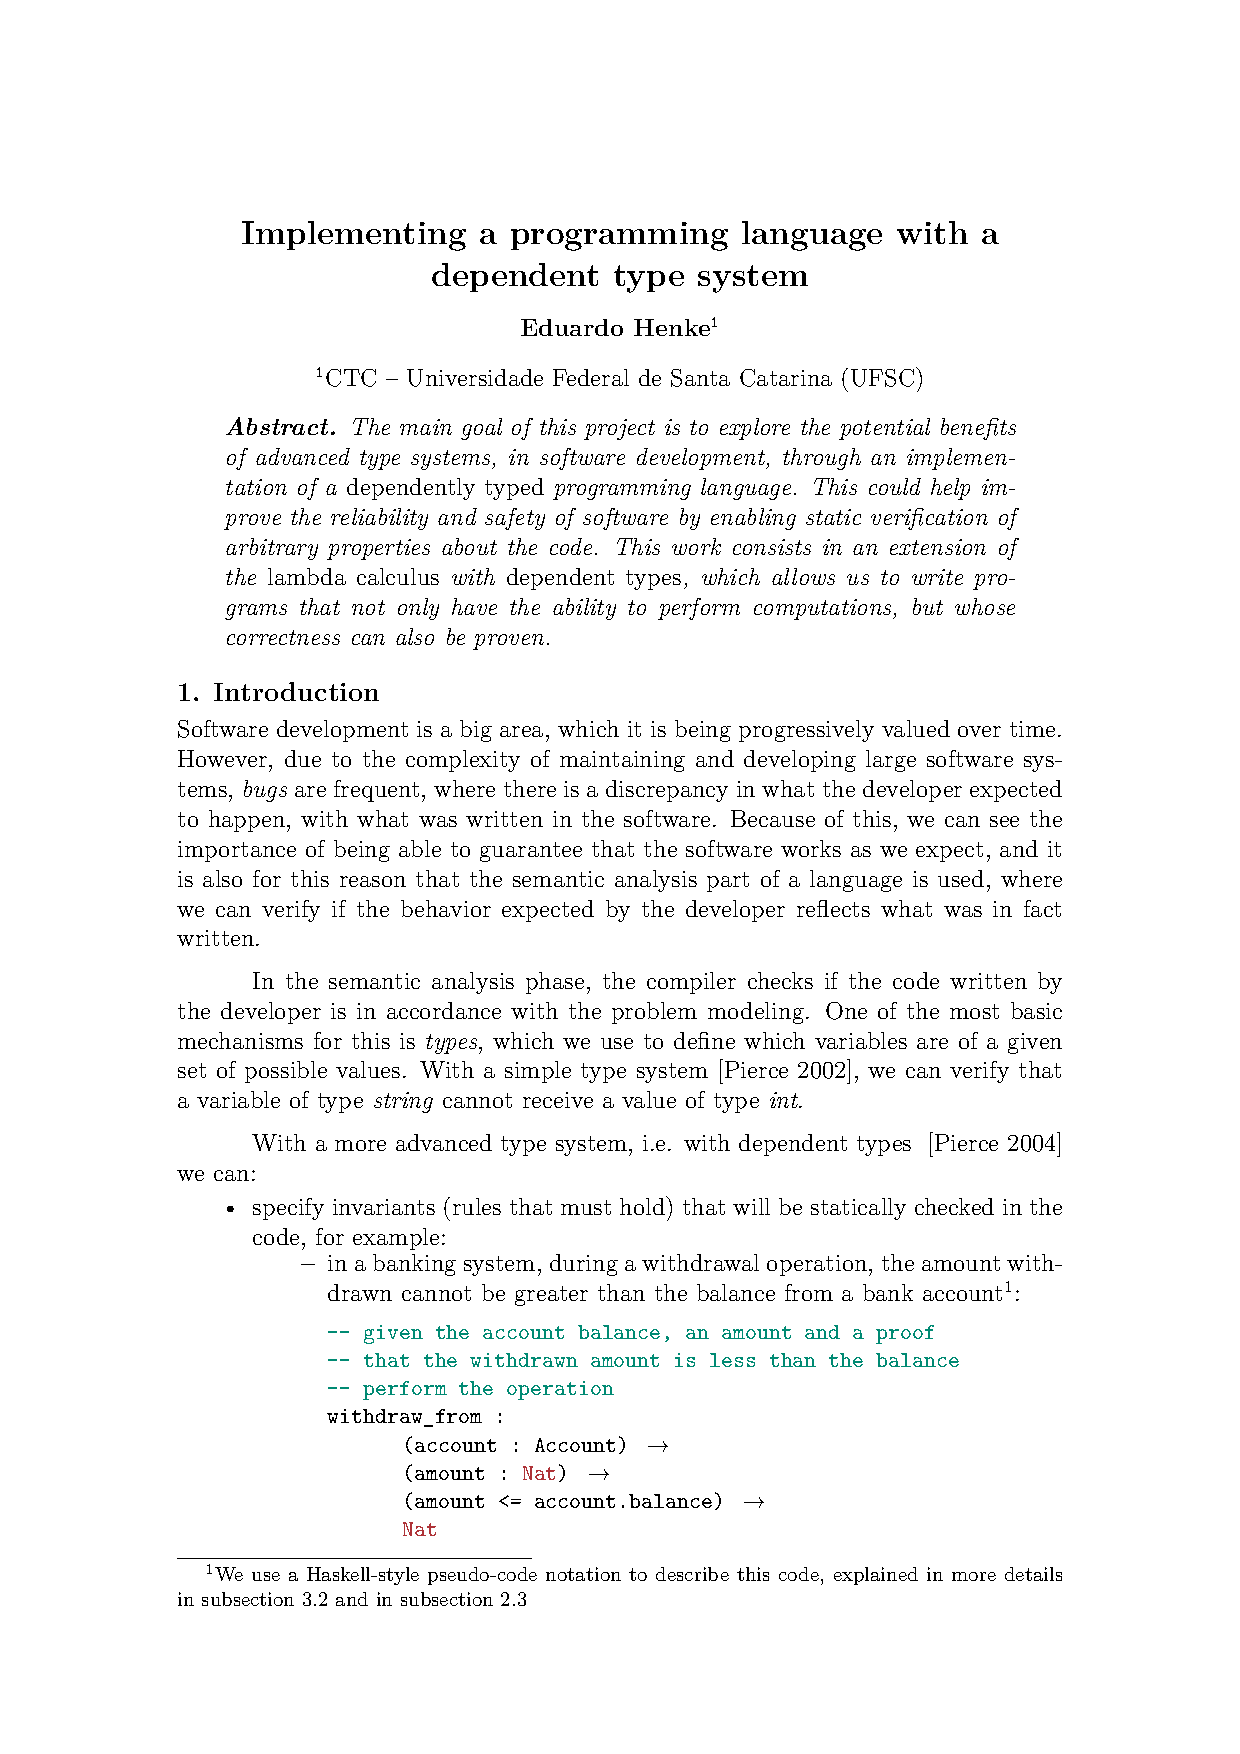
\includepdf[pages=1-]{paper/paper.pdf}

\end{document}